The purpose of this algorithm is to make a 3D tracking object, producing position informations 
about the followed target.
These informations will be relevant to define parameters 
as: the relative velocity, the factor of approaching and of departure.

The proposed algorithm begin with a key frame image where a initial Region Of Interest ($ROI$) is determined; 
the system then receive a stream of image frames and the tracking system 
enters in looping to follow the target in the frames as is shown in the Fig. \ref{fig:system}.


\begin{figure}[bhp]
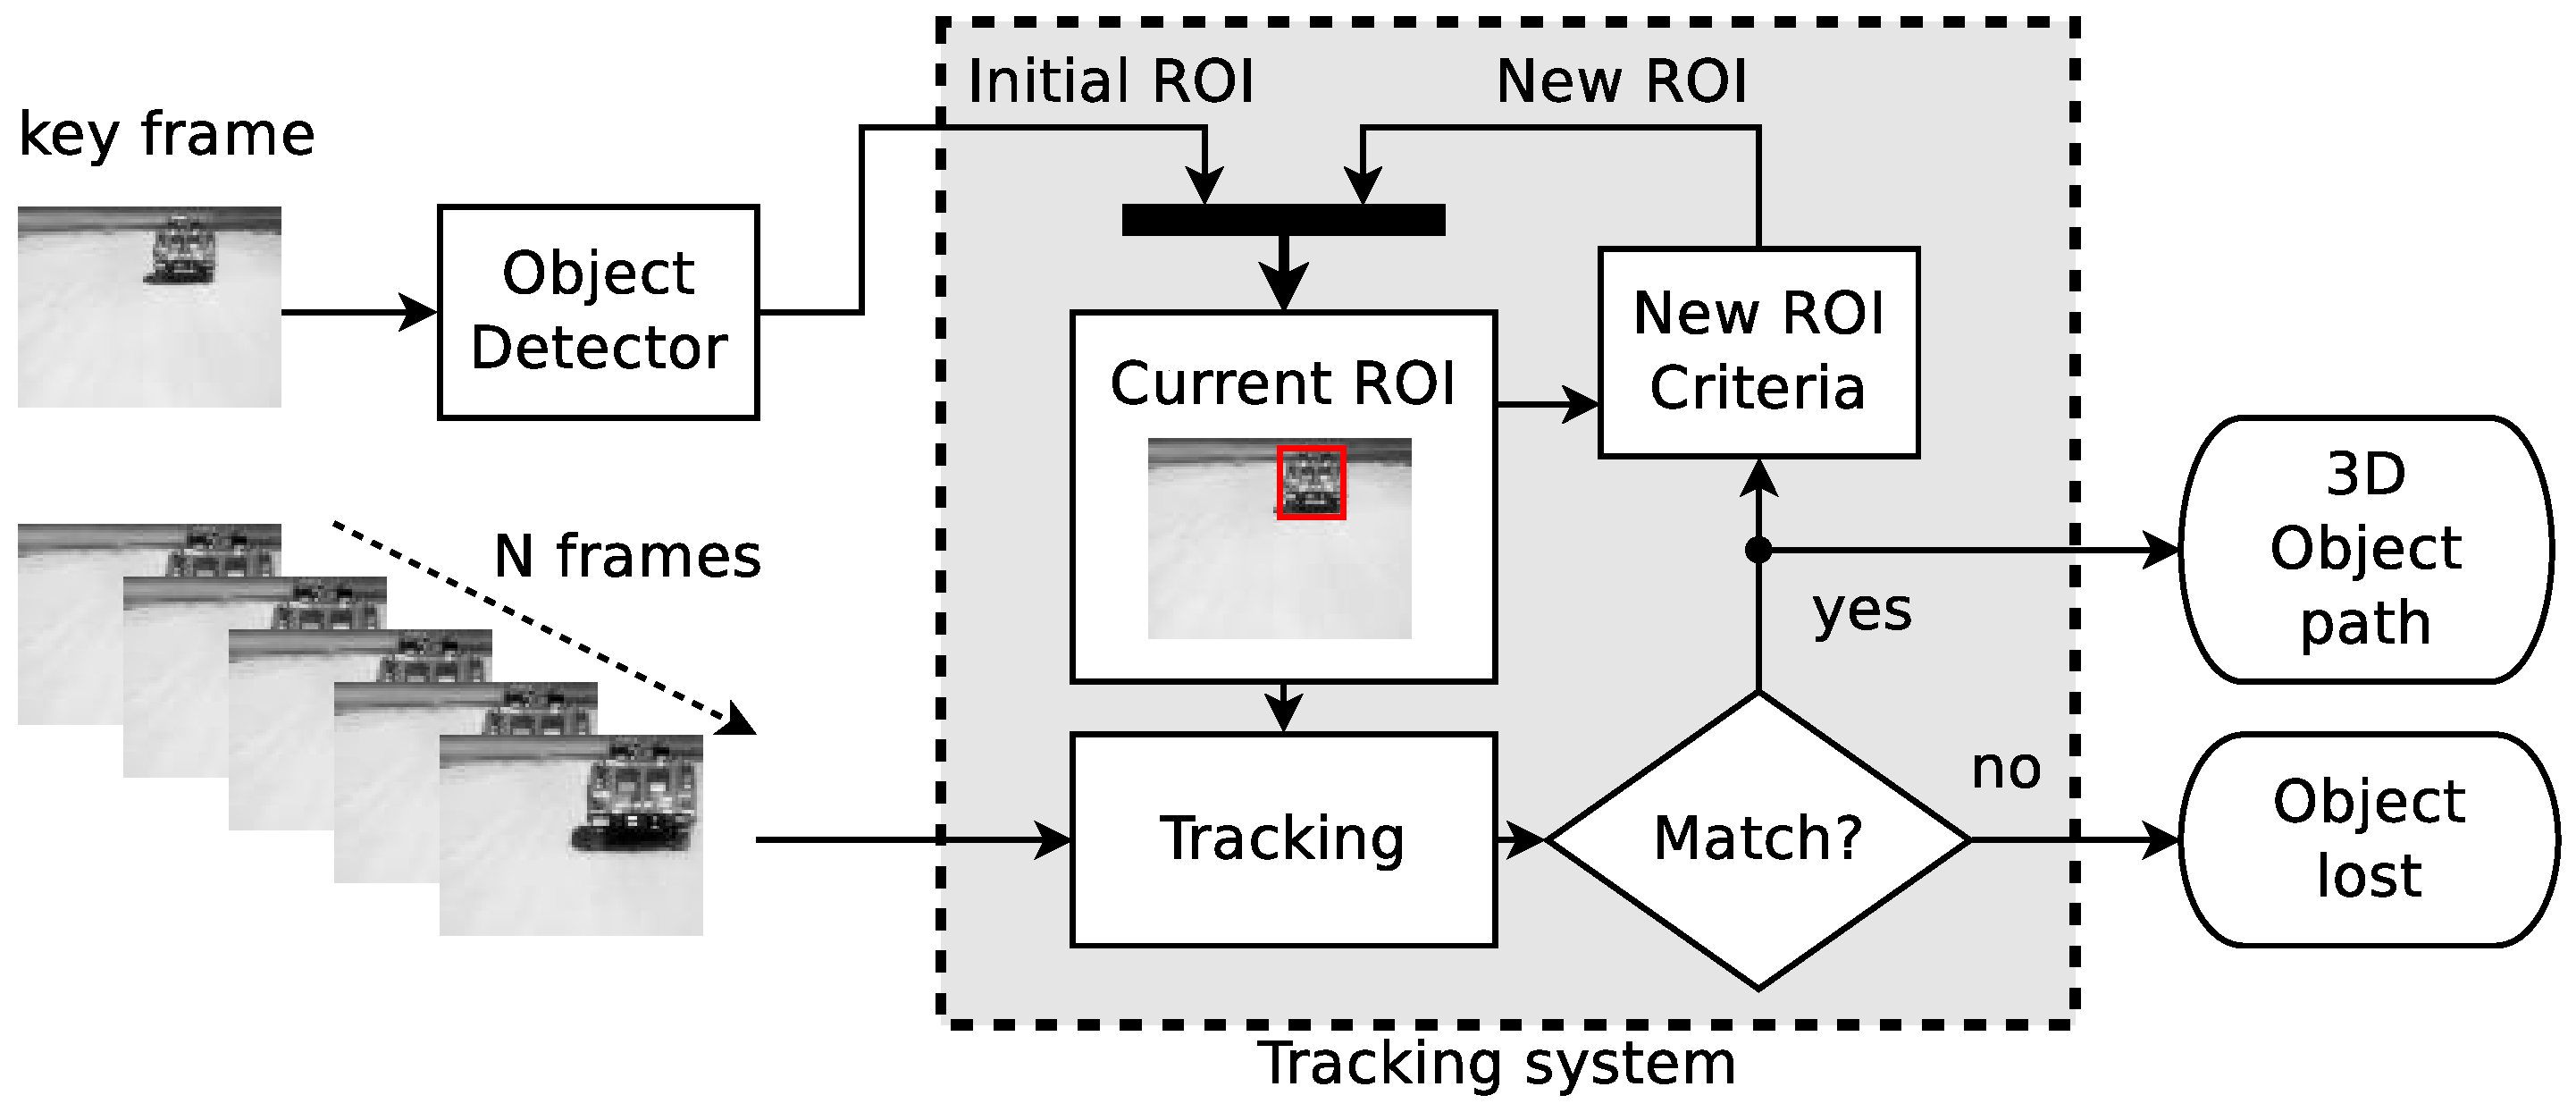
\includegraphics[width=\columnwidth]{images/figure1-diagram1.eps}
\caption{With the current $ROI$ selected, a highest value of $PCC$, between the $ROI$ 
and the Window Of Search ($WOS$) of current frame, identifies the target; 
the result of search is a displacement vector
between the first and last position of object. 
After, this processing is made again to the next frames.}
\label{fig:system}
\end{figure}

In a 2 dimensional analysis, the tracked objects given us information about your horizontal 
and vertical position, and your relative perpendicular velocity respect to the observer.
When the target is analyzed in 3 dimensions, 
the initial $ROI$ has the position $(x=x_0,y=x_0,d=d_0=1)$;
where, $x_0$ and $y_0$ represent a position (horizontal and vertical) in the analyzed image,
and $d_0=1$ represents the initial depth position of object in the $ROI$ (normalized by definition to $1.0$).
Thus, all the results of depth will be relatives to this value, 
In this sense only can be calculated relative values of
velocity and the factor of approaching or departure. 

%Diagrama1
 %A gente vai explicar o algoritmo como uma caixa fechada , que coisa entra e que coisa sai
 %e os parametros a sintonizar.
 % como usar ele quando implementado, como se fosse uma caixa preta.
